\section{Stacks}
\label{sec:stacks}

\begin{frame}
	\frametitle{Stacks}
	\begin{center}
		
\includegraphics[width=0.4\textwidth]{figures/stack_of_books.png}\\
		\hspace*{15pt}\hbox{\scriptsize Image from \thinspace{\itshape Pixabay}}
		% https://pixabay.com/en/books-stacked-pile-stacks-25159/
	\end{center}
\end{frame}

\begin{frame}
	\frametitle{Me and my books}
	\framesubtitle{A life-long story}

	\begin{columns}
		\column{0.455\textwidth}
			\begin{center}
				\alt<4->{
					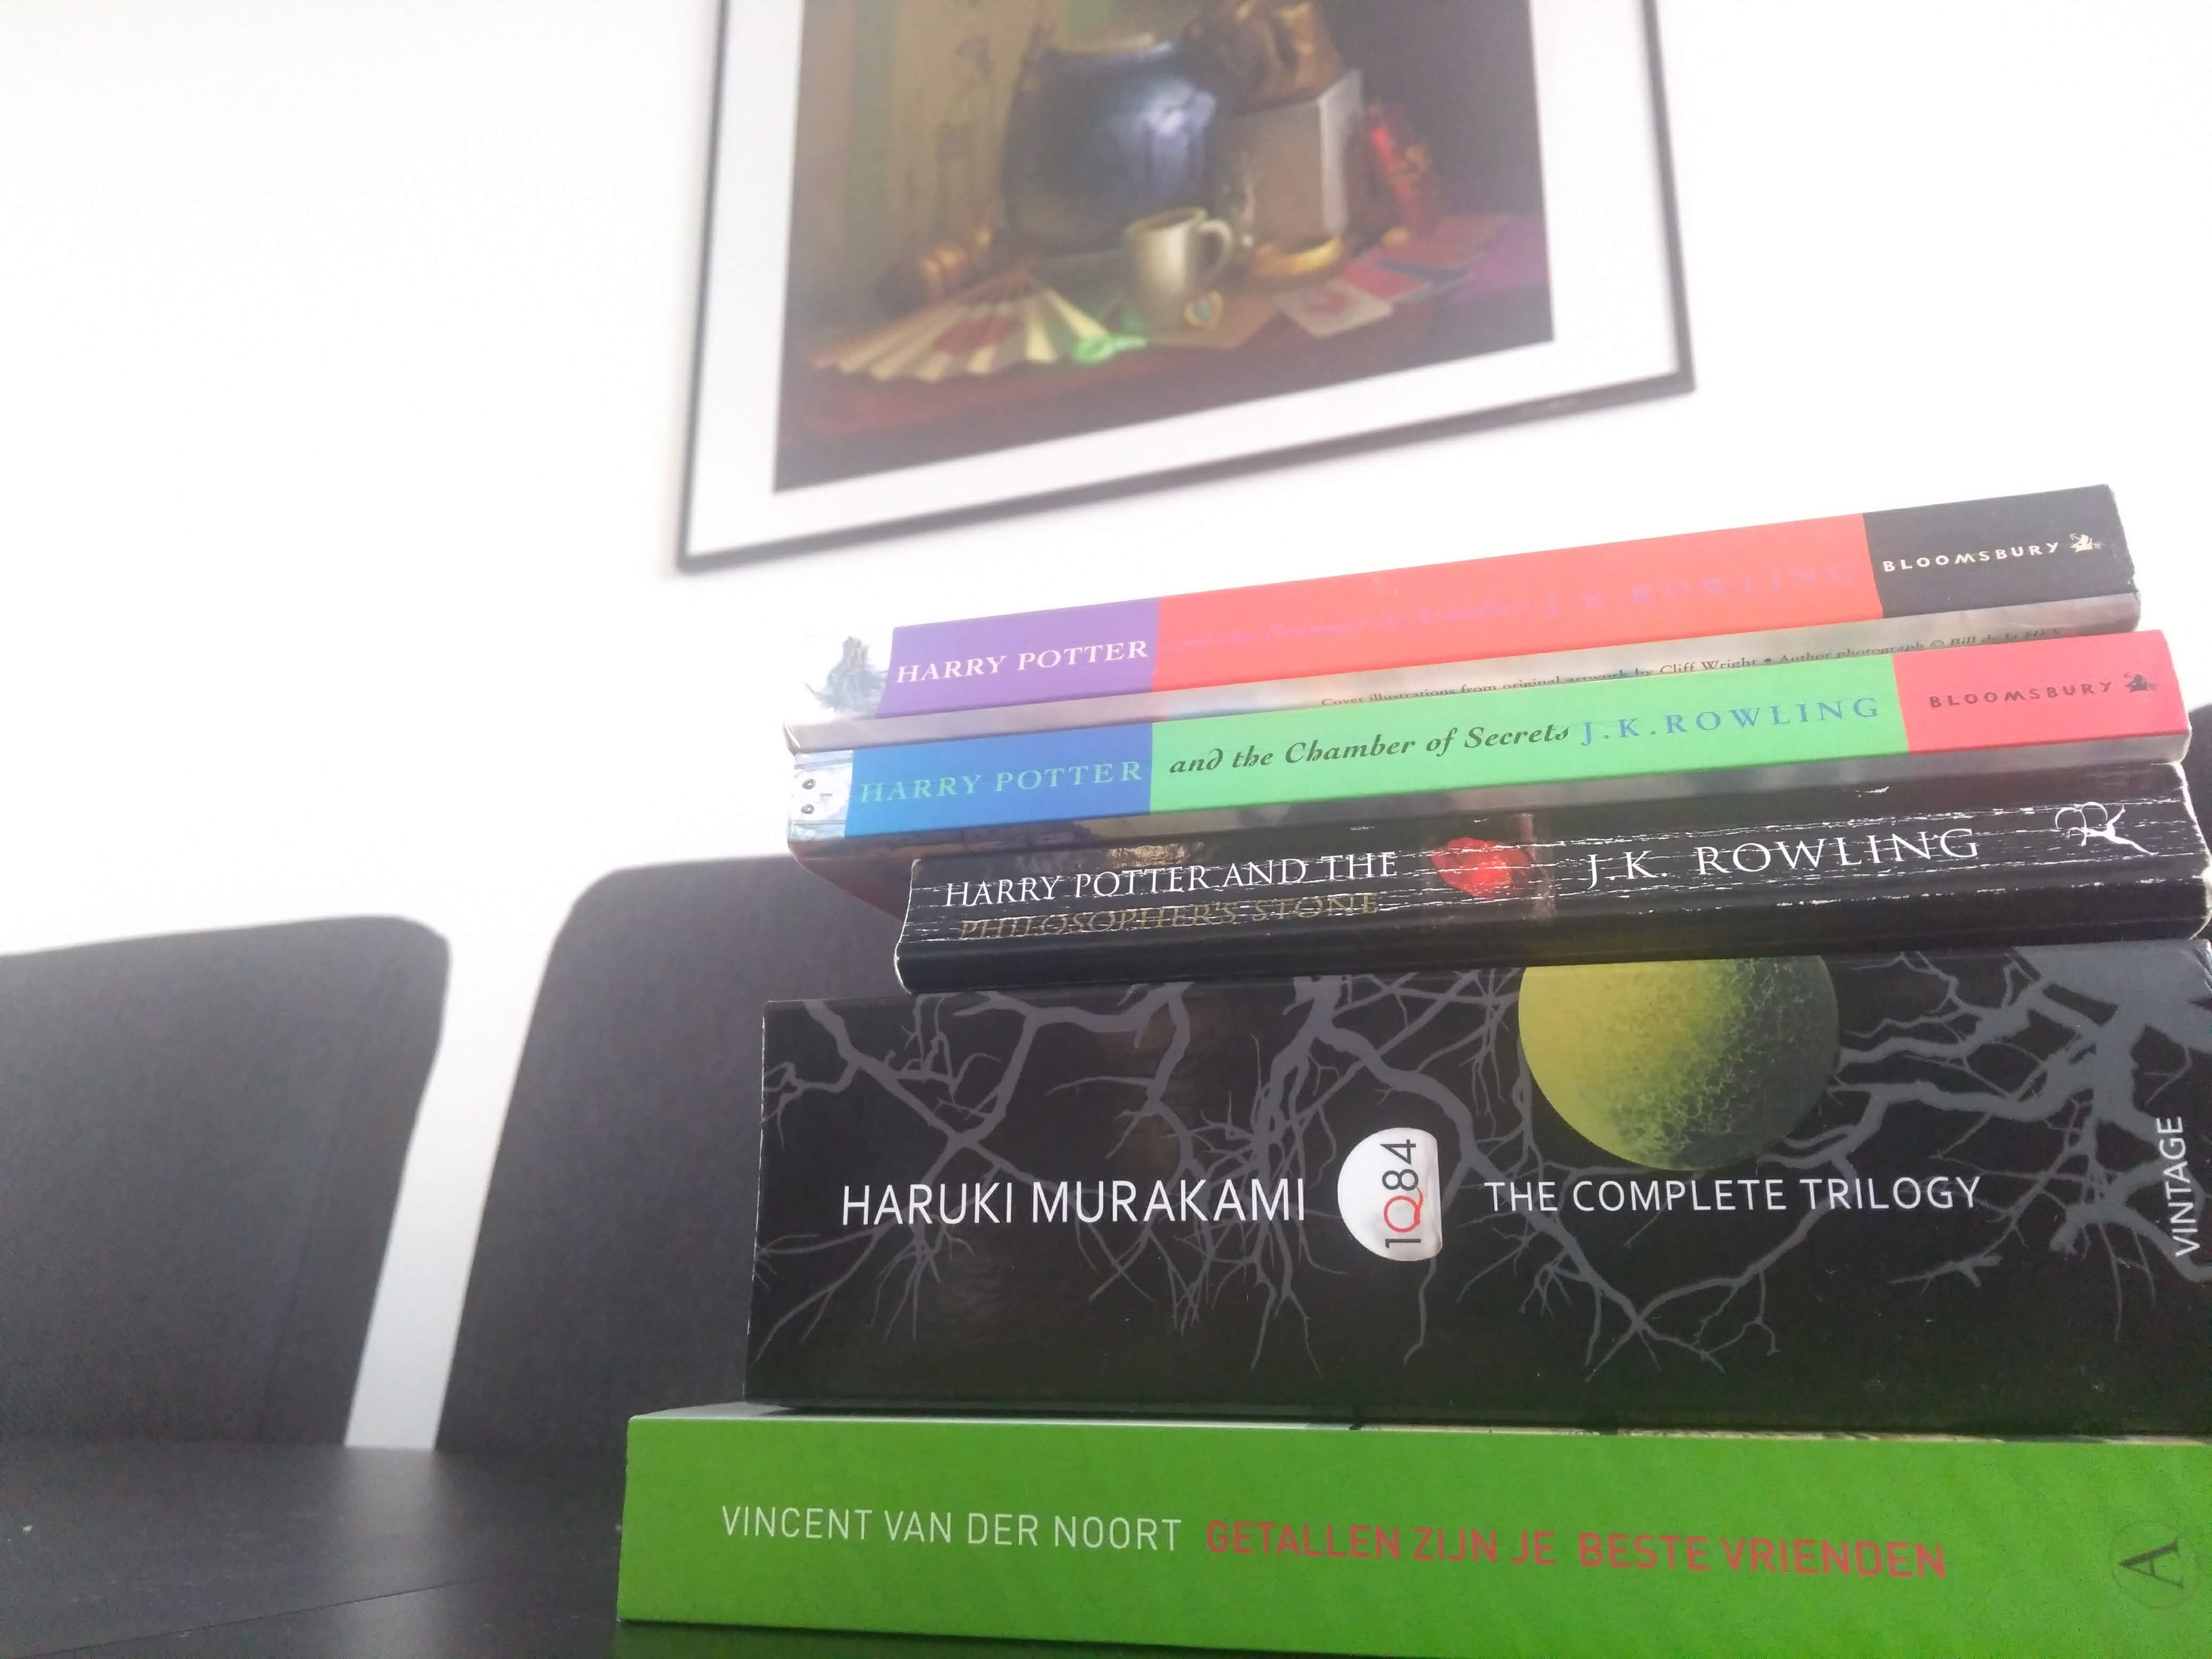
\includegraphics[width=\textwidth]{figures/stack_read.jpg}\\
					}{
					
\includegraphics[width=\textwidth]{figures/stack_unread.jpg}\\
					}
				\hspace*{15pt}\hbox{\scriptsize Image By:\thinspace{\itshape Stefan Hugtenburg}}
				\hspace*{15pt}\hbox{\scriptsize Bookcovers and picture in the back by others}
			\end{center}
		\column{0.455\textwidth}
		\begin{itemize}
			\item This is how I used to store books I still wanted to read.
				\pause
			\item A nice \alert{stack} of books, with new ones going on the top.
				\pause
			\item After finishing one, I would take the next one from the top.
				\pause
			\item So after a few weeks\dots
				\pause
			\item This uses the \alert{LIFO}-principle.
		\end{itemize}
	\end{columns}
\end{frame}

\begin{frame}
	\frametitle{The what!?}
	\framesubtitle{LIFO}
	
		\begin{block}{LIFO}
			The \textit{Last-In-First-Out}, or LIFO, principle is the working of a stack.\\
			\pause
			The last thing we've added to the stack is the first thing we take out.\\
			\pause
			Similarly the first we have added to the stack, is the last to be taken out.
		\end{block}	
\end{frame}

\begin{frame}
	\frametitle{The Stack ADT}
	\begin{overlayarea}{\textwidth}{\textheight}
		\only<1>{
			\begin{block}{ADT}
				An ADT, or Abstract Data Type, is a description of the behaviour of a data structure.
			\end{block}	
		}
		\pause
			\begin{block}{The Stack}
				\begin{itemize}
					\item \texttt{size()} (or \texttt{len(s)}) to get the number of items in the stack.
					\item \texttt{push(item)} to add something to the stack.
						\pause
					\item \texttt{pop()} to remove the top element from the stack.
					\item \texttt{top()} to view the top element of the stack.
				\end{itemize}
			\end{block}	
			\pause
			\begin{questionblock}{Data structure?}
				What kind of data structure should we use to implement a Stack?
				\only<4>{
				\begin{enumerate}[A.]
					\item An array
					\item A python list
					\item A linked list
					\item A dict
				\end{enumerate}
			}
			\end{questionblock}
			\pause
			\begin{answerblock}{One end only}
				Only removing and adding on one end? Seems like a DLL will do.
			\end{answerblock}
	\end{overlayarea}
\end{frame}

\begin{frame}
	\frametitle{Implementing a Linked-List based Stack}
	\begin{overlayarea}{\textwidth}{\textheight}
			\begin{tabular}{r | c c}
				Stack operation & DLL operation & Time Complexity \\
				\midrule
				\texttt{size} & \only<2->{\texttt{size} & $O(1)$} \\
				\texttt{push} & \only<2->{\texttt{add\_last} & $O(1)$} \\
				\texttt{pop}  & \only<2->{\texttt{remove\_last} & $O(1)$} \\
				\texttt{top}  & \only<2->{\texttt{tail} & $O(1)$} \\
			\end{tabular}
		
			\begin{columns}[t]
				\column{0.455\textwidth}
			\only<3->{
			\begin{questionblock}{Arrays}
				Could we also do this using an array-based list?	
			\end{questionblock}
		}
			\only<5->{
			\begin{questionblock}{SLL}
				What about an SLL?
			\end{questionblock}
		}
				\column{0.455\textwidth}
				\only<4->{
				\begin{answerblock}{Amortised}
					Sure, but it's only amortised $O(1)$. So why would we?
				\end{answerblock}
				}
				\only<6->{
				\begin{answerblock}{Front = Back}
					Sure, but we add and remove from the front!
				\end{answerblock}
				}
		
			\end{columns}
	\end{overlayarea}
\end{frame}

